\documentclass{article}
\usepackage{dtrt}
\usepackage{graphicx} % Required for inserting images
\usepackage{fontspec}
\usepackage{libertine}
\usepackage{enumitem}
\usepackage{fullpage}
\usepackage{tikz}
\usetikzlibrary{arrows.meta, shapes.geometric, positioning, fit, backgrounds, calc}

% BibTeX configuration
% Format: BMS24 style (author initials + two-digit year, e.g., [BMS24])
\bibliographystyle{alpha}
\setlength{\parindent}{0pt} % No indentation for paragraphs
\setlength{\parskip}{0.5em} % Add gap between paragraphs

\title{Private Information Retrieval for Bitcoin Light Clients}
\author{Weikeng Chen}
\date{March 2026}

\begin{document}

\maketitle

\section{Introduction}

We are interested in using Private Information Retrieval (PIR) to help Bitcoin light clients synchronize with the Bitcoin network that suffices to enable the light clients to identify and spend their UTXOs. 

\subsection{Selections of PIR protocols}

We are interested in four settings: 
\begin{itemize}[nolistsep,leftmargin=*]
    \item \textbf{Single-server:}
    \smallskip
    \begin{itemize}[nolistsep,leftmargin=*]
        \item Almost no client storage: YPIR-over-SimplePIR \cite{ypir2024}

        \item Sublinear client storage without a linear pass: SimplePIR or DoublePIR \cite{henz23}

        \item Sublinear client storage after a linear pass: Plinko \cite{plinko2024}, RMS24 \cite{rms24}, or Piano \cite{piano2024}
    \end{itemize}

    \smallskip
    \item \textbf{2-server:}
    \smallskip
    \begin{itemize}[nolistsep,leftmargin=*]
        \item Almost no client storage: DPF-PIR \cite{gilboa2014dpf,boyle2015fss,boyle2016fss}

        \item Sublinear client storage: Plinko, RMS24, or Piano but moving the hint generation to a hint server
    \end{itemize}
\end{itemize}

\textbf{Single-server.} We focus on single-server PIR without per-client storage on the server and allow server to preprocess the database. For protocols that do not require client storage (or if the client storage is just for some data-independent parameters), YPIR-over-SimplePIR has achieved best performance and throughput for larger blocks, in comparison to Hintless PIR \cite{li24}, Tiptoe \cite{tiptoe23}, and Spiral \cite{spiral22}. 

If we allow the client to make data-dependent but sublinear storage for ``hints'', then we get better results with SimplePIR or DoublePIR, where the client downloads the hints before making any query. Note that DoublePIR is most suitable for single-bit or few-bit entries, and does not perform well when the entry size exceeds several tens of bits. This is because: (1) while the client hint is independent of the database size, it scales linearly with the entry size; and (2) this linear scaling has a very large multiplicative constant factor. This makes DoublePIR suitable for certain PIR use cases, but not the other. When using SimplePIR or DoublePIR, the server time appears to improve around $2$ times to an order of magnitudes with the sublinear hints over those that don't require hints.

If we do one step further and allow the client to download and make a linear pass over the database to generate sublinear hints (the client downloads and performs the linear pass in the streaming manner with only sublinear storage needed), then we can get much better performance with Plinko, RMS24, or Piano. The server time can be reduced by potentially two orders of magnitude. This setting works well for many devices with access to home internet or WiFi network where the network is not metered, but not all. 

\textbf{2-server.} We now consider PIR that assumes two servers that are non-colluding and non-communicating, meaning that the two servers do not need to know each other, and it is only the user who engages with both servers. In fact, any two trustworthy servers that have the database can be selected by the user to run this protocol. This setting is especially relevant to Bitcoin peer-to-peer (P2P) network as a user can discover two full nodes that provide this capability and use their help. The caveat is that the user needs to trust that these two servers do not collude with each other. If not, the two colluding servers can immediately learn the user's query.

The easiest way to achieve 2-server PIR is to use DPF-PIR, which is based on distributed point functions (DPF) \cite{gilboa2014dpf,boyle2015fss,boyle2016fss}. Given a share of DPF keys of size $O(logN)$, each server can expand it to $N$ bits that look random, where the two servers' bits differ exactly on the location that the user queries. Each server retrieves the entries with bit $1$ and computes an XOR sum of them. The user finally performs an XOR over the two XOR sums from the two servers and obtains the desired query result. It requires $O(NB)$ server compute time with $B$ being the entry size, but the computation is extremely lightweight. Usually, the compute can answer a PIR query close to the time that it takes to do a linear pass of the database in the storage medium (which usually is the main memory).

If we allow hint generation, as is the case in the single-server setting, we know that the server can answer the PIR queries in sublinear time, which is extremely efficient that seems to ``surpass the memory speed.'' Previously in the single-server setting, a significant downside is that the client needs to download the entire database (in a streaming manner) to generate the hint locally. Now, in the 2-server setting, the user can outsource the hint generation to one of the servers (``hint server''), and the hint can be used to query any server other than the hint server. This avoids the need for the user to download the database, and the user can directly download the hint, though it still requires sublinear client storage.

\textbf{How many queries would a user make?} When we compare these different solutions, it is important to understand how many queries a user would make. For example, if a user only makes one query, then all the compute and communication costs for the hint generation may not be worthwhile if it is single-use. The overhead is not just about the client, but also the server. For single-server protocols that require a linear pass, a server needs to serve the entire database to this user. For 2-server protocols with outsourced hint generation, the hint server bears the computation cost for doing that linear pass over its local copy of the database.

This is especially relevant to Bitcoin light client synchronization because a light client may maintain a small wallet that only cares about UTXOs that the wallet can spend. In this situation, the light client knows exactly how many queries it needs to make, and after those queries, the light client has no need to access this database anymore as it has been synced up to the state that is current to the database. In this case, the client may only make one or a few queries to the database, and therefore the overhead for hint generation may not be worthwhile. An example of such a use case is when a light client imports a seed phrase or a private key, in which case it needs to identify all the UTXOs associated with the imported wallets, but this is a one-time thing. 

Despite this concern, PIR is still superior than asking the light client to download the compact block filters for all the blocks since the imported key is first used (if known) and fetch a  number of blocks. First, the compact block filters for the entire Bitcoin history can still be a few gigabytes. Second, the usual way to fetch relevant blocks is to request these blocks directly from a full node by giving the block height, which leaks a little bit of privacy (which blocks this new wallet has a UTXO for). Whether this privacy leakage is acceptable depends on the situation and the user. Our goal building the PIR solution is to help those users who want to avoid this privacy leakage (which, as we will show, it is easy to avoid).

\textbf{Malicious security.} Modern PIR naturally achieves privacy even against malicious servers, so we only need to focus on integrity. There are many ways to achieve integrity, some of which offer integrity against selective failure attacks \cite{kilian88,naor99,dwork99,camenisch07,lindell11,kiraz06}, while some do not. Whether it is okay to ignore selective failure attacks depends on the user and the use case. For example, a user who receives a potentially selectively failed response can continue to finish the rest of the protocol using random queries, pretending to have received a valid response, and then fetch the data from other servers.

If we ignore selective failure attacks, the most practical solution for single-server and 2-server solutions appears to be KZG polynomial commitment \cite{kzg10}, where the opening proofs are generated using the Feist-Khovratovich batch technique \cite{fk23}. An important limitation is that it uses elliptic curves, and therefore is not post-quantum. The KZG opening proof would add about 16 bytes to each entry. To reduce the PIR compute overhead caused by the additional opening proof, we can merge a few entries into one larger entry, and still only one opening proof is needed for the larger entry. With the same setup parameters of KZG, all the nodes in the network should have the same KZG polynomial commitment. 

This solution, however, fails to address selective failure attacks. Selective failure attacks refer to the case when a malicious server manipulates a subset $S$ of the database entries such that if the user is reading an entry in $S$, it would fail, and if the user is reading an entry outside of $S$, it would succeed. The concern is that such a selective failure, which may be realized by the malicious server through a change of the user's subsequent actions, can leak if the user is reading an entry in $S$.

To address selective failure attacks, we can choose protocols with this additional verifiability guarantee against selective failure attacks. For single-server protocols without a linear pass, RLP26 \cite{rlp26} is a good candidate, which improves over VeriSimplePIR \cite{cl24} and significantly reduces the client hint using some one-time computation. 
\begin{itemize}[nolistsep,leftmargin=*]
    \item \textbf{Single-server:}
    \smallskip
    \begin{itemize}[nolistsep,leftmargin=*]
        \item Almost no client storage: RLP26 \cite{rlp26}

        \item Sublinear client storage after a linear pass: Plinko, RMS24, or Piano with Merkle proofs, or verifiable BALANCED-PIR \cite{ar26}
    \end{itemize}

    \smallskip
    \item \textbf{2-server:} Plinko, RMS24, or Piano with Merkle proofs, or verifiable BALANCED-PIR with outsourced hint generation
\end{itemize}


\section{PIR for UTXO set}

A light client knowing a receiving ScriptPubKey can use PIR to pull TXID + vout + amount of an UTXO under that ScriptPubKey. This is basically all a light client needs to know in order to spend this UTXO.

\begin{figure}[htbp]
\centering
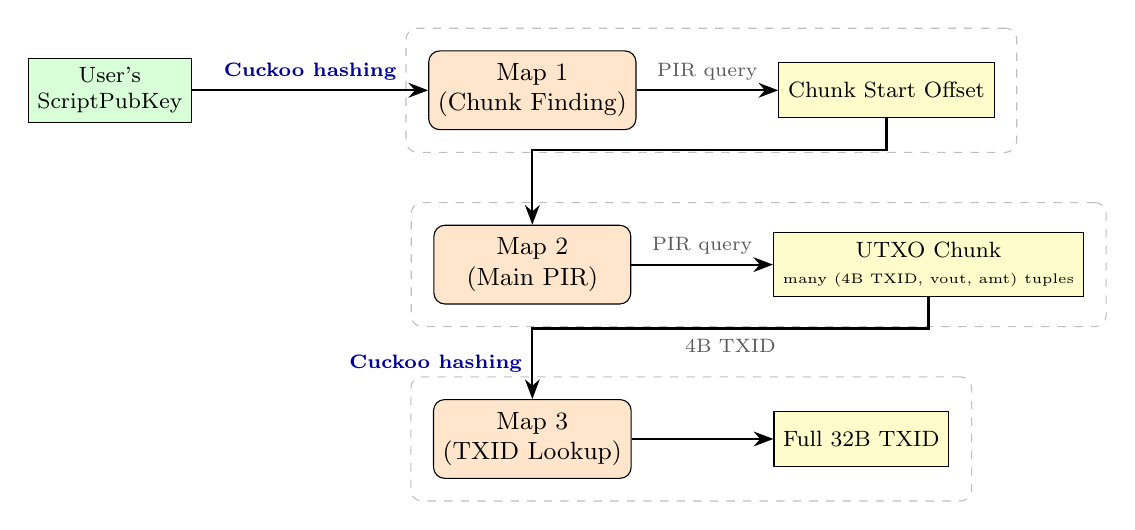
\begin{tikzpicture}[
    node distance=1.2cm and 1.8cm,
    box/.style={rectangle, draw, rounded corners, minimum width=2.5cm, minimum height=1cm, align=center, font=\small},
    data/.style={rectangle, draw, fill=blue!10, minimum width=1.8cm, minimum height=0.7cm, align=center, font=\footnotesize},
    arrow/.style={-{Stealth[length=2.5mm]}, thick},
    label/.style={font=\scriptsize, text=gray!70!black},
    pirlabel/.style={font=\scriptsize\bfseries, text=blue!60!black}
]

% Row 1: User input -> Map 1 -> Chunk Index + Offset
\node[data, fill=green!15] (user) {User's\\ScriptPubKey};

\node[box, fill=orange!20, right=3cm of user] (map1) {Map 1\\(Chunk Finding)};

\node[data, fill=yellow!20, right=of map1] (chunkidx) {Chunk Start Offset};

% Row 2: Map 2 -> UTXO Chunk
\node[box, fill=orange!20, below=of map1] (map2) {Map 2\\(Main PIR)};

\node[data, fill=yellow!20, right=of map2] (utxo) {UTXO Chunk\\{\tiny {many (4B TXID, vout, amt) tuples}}};

% Row 3: Map 3 -> Full TXID -> Output
\node[box, fill=orange!20, below=of map2] (map3) {Map 3\\(TXID Lookup)};

\node[data, fill=yellow!20, right=of map3] (fulltxid) {Full 32B TXID};

% Arrows - Row 1
\draw[arrow] (user) -- (map1) node[midway, above, pirlabel] {Cuckoo hashing};
\draw[arrow] (map1) -- (chunkidx) node[midway, above, label] {PIR query};

% Arrow from Chunk Index down to Map 2
\draw[arrow] (chunkidx.south) -- ++(0,-0.4) -| (map2.north);

% Arrows - Row 2
\draw[arrow] (map2) -- (utxo) node[midway, above, label] {PIR query};

% Arrow from UTXO down to Map 3
\draw[arrow] (utxo.south) -- ++(0,-0.4) -| (map3.north) node[near start, below, label] {4B TXID} 
node[near end, left, pirlabel] {Cuckoo hashing};

% Arrows - Row 3
\draw[arrow] (map3) -- (fulltxid);

% Labels for the maps

% Background boxes for grouping
\begin{scope}[on background layer]
    \node[fit=(map1)(chunkidx), draw=gray!50, dashed, rounded corners, inner sep=8pt, label={[font=\tiny\itshape, text=gray]above:Step 1}] {};
    \node[fit=(map2)(utxo), draw=gray!50, dashed, rounded corners, inner sep=8pt, label={[font=\tiny\itshape, text=gray]left:Step 2}] {};
    \node[fit=(map3)(fulltxid), draw=gray!50, dashed, rounded corners, inner sep=8pt, label={[font=\tiny\itshape, text=gray]left:Step 3}] {};
\end{scope}

\end{tikzpicture}
\caption{Overview of the three PIR maps for UTXO lookup. The user starts with a ScriptPubKey and retrieves the complete UTXO information through a sequence of three map lookups.}
\label{fig:three-maps}
\end{figure}

\textbf{Sort and group.} The server prepares the database by sorting them by ScriptPubKey, then secondarily sorted by the TXID (descending), and grouping them into continuous chunks. A user may need to query multiple chunks if the user is behind in the sync, but we expect most of the users (who occasionally make transactions) only need to read the first chunk. The TXID would be remapped to a 4-byte integer, which is the index of a TXID, sorted by how early they appear in the entire Bitcoin chain, which is unique and unchanged, with delta encoding and VarInt. A chunk can consist of data from multiple ScriptPubKeys. In YPIR-over-SimplePIR and SimplePIR, it is possible to make it easy for a user to read continous range of chunks through the native batching occurring in the SimplePIR protocol by placing the continuous chunks carefully in the matrix.

\textbf{Map ScriptPubKey to chunk's start offset.} The server maintains another database that maps the ScriptPubKey to the chunk's start offset in the database. This is the common PIR-by-keyword setting and can be generally supported by Cuckoo hashing \cite{PR01}. The response would be dominated by a hash of the ScriptPubKey and the chunk's start offset. It is necessary to include a hash of the ScriptPubKey because a client may query a ScriptPubKey that has no presence in the database (for example, no incoming transactions to a newly created address).

\textbf{Map 4-byte TXID to full 32-byte TXID.} A user needs to remap the 4-byte TXID back to the full 32-byte TXID. Generally, this map only cares about TXIDs in the UTXO set, and therefore only a small subset of all the TXID in the Bitcoin chain needs to be included here. Therefore, it seems always helpful to apply a layer of Cuckoo hashing.

\textbf{Batch PIR.} We can apply the idea of batch PIR \cite{IKOS04} to all these constructions, which would opportunistically reduce the overall cost when querying multiple entries at the same time. One can go with the simple ``opportunistical'' batching in SimplePIR, but it is also possible to apply an actual layer of batch codes as in the SealPIR paper \cite{sealpir18}.
\begin{itemize}[nolistsep,leftmargin=*]
    \item For YPIR-over-SimplePIR and DPF-PIR, it can opportunistically reduce the average compute cost by a factor of $o(k)$ for the server.

    \item For other constructions, it can opportunistically save $o(\sqrt{k})$ in communication and compute, but mind that the hints dedicated for batch PIR to fetch $k$ queries, if used on just one single query, would increase a $O(\sqrt{k})$ factor of waste.
\end{itemize}


\textbf{Distributional PIR.} We can potentially apply the idea of distributional PIR \cite{lehmkuhl25} to further reduce the average cost for the target users that use a light client. The idea of distributional PIR is to note that some entries in the database are more likely going to be queried than others, and the PIR algorithm can be tuned to optimize for the more likely queries at the cost of slowing down the less likely queries. This works for the Bitcoin light client setting because older UTXOs may be less likely of interest and ScriptPubKeys with a large number of UTXOs may be a very active address that probably has been running a full node themselves (e.g. crypto exchange). Moreover, non-Taproot ScriptPubKeys are mostly from older clients rather than newer clients who might probably be using PIR. The benefit of distributional PIR is that it does not rule out the ability to query these less likely entries, but it just makes them slightly slower. This would end up beneficial to all users as the average cost for the server is lower, allowing a busy server to respond to more queries at a lower cost. 

\section{Implementation}

We have implemented a complete, production-ready system based on the DPF-PIR approach described in Section 2. The implementation consists of three main components: database generation tools, PIR servers, and client libraries. The system is designed to support the three-map architecture illustrated in Figure~\ref{fig:three-maps}.

\subsection{System Architecture}

The implementation follows a two-server architecture where each server maintains an identical copy of the databases and operates independently. The client connects to both servers via WebSocket and distributes DPF keys to each server, ensuring that neither server learns the query target as long as they do not collude.

\begin{figure}[htbp]
\centering
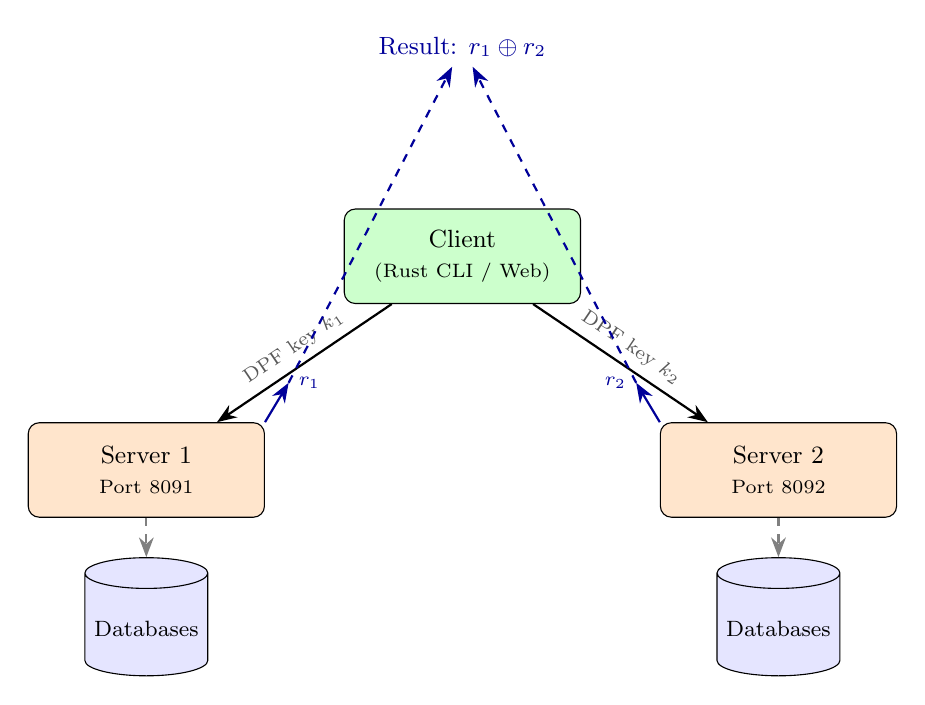
\begin{tikzpicture}[
    node distance=1.5cm and 2cm,
    box/.style={rectangle, draw, rounded corners, minimum width=3cm, minimum height=1.2cm, align=center, font=\small},
    db/.style={cylinder, draw, shape border rotate=90, aspect=0.25, minimum height=1.5cm, minimum width=1.2cm, fill=blue!10, font=\footnotesize},
    arrow/.style={-{Stealth[length=2.5mm]}, thick},
    label/.style={font=\scriptsize, text=gray!70!black}
]

% Client
\node[box, fill=green!20] (client) {Client\\{\scriptsize (Rust CLI / Web)}};

% Servers
\node[box, fill=orange!20, below left=1.5cm and 1cm of client] (server1) {Server 1\\{\scriptsize Port 8091}};
\node[box, fill=orange!20, below right=1.5cm and 1cm of client] (server2) {Server 2\\{\scriptsize Port 8092}};

% Databases
\node[db, below=0.5cm of server1] (db1) {Databases};
\node[db, below=0.5cm of server2] (db2) {Databases};

% Connections
\draw[arrow] (client) -- (server1) node[midway, above, sloped, label] {DPF key $k_1$};
\draw[arrow] (client) -- (server2) node[midway, above, sloped, label] {DPF key $k_2$};
\draw[arrow, dashed, gray] (server1) -- (db1);
\draw[arrow, dashed, gray] (server2) -- (db2);

% Response
\draw[arrow, blue!60!black] (server1.north east) -- ++(0.3, 0.5) node[right, font=\scriptsize] {$r_1$};
\draw[arrow, blue!60!black] (server2.north west) -- ++(-0.3, 0.5) node[left, font=\scriptsize] {$r_2$};

% XOR
\node[above=1.8cm of client, font=\small, text=blue!60!black] (xor) {Result: $r_1 \oplus r_2$};
\draw[arrow, blue!60!black, dashed] ($(server1.north east)+(0.3, 0.5)$) -- (xor);
\draw[arrow, blue!60!black, dashed] ($(server2.north west)+(-0.3, 0.5)$) -- (xor);

\end{tikzpicture}
\caption{Two-server DPF-PIR architecture. The client generates two DPF keys from the query index and sends one to each server. The servers compute XOR sums over their databases, and the client combines the responses to recover the result.}
\label{fig:architecture}
\end{figure}

\subsection{Database Generation Pipeline}

The database generation pipeline transforms raw Bitcoin blockchain data into the three PIR-queryable databases. This offline process is run periodically to update the servers with the latest UTXO set. The pipeline consists of eight sequential stages, each implemented as a separate Rust binary in the \texttt{build\_db/src/bin} directory. Common functionality---duration and byte formatting, MPHF loading, progress file management, and TXID skip lists---is shared through a \texttt{utils} module in the library crate to avoid duplication across stages.

\subsubsection{Stage 1: TXID File Generation (\texttt{gen\_1\_txid\_file.rs})}

The pipeline begins by extracting all transaction IDs from Bitcoin's block data files. We use the \texttt{brk\_reader} library for high-performance block parsing, which directly reads the \texttt{blk*.dat} files rather than relying on slower RPC calls.

\textbf{Input:} Bitcoin Core data directory containing \texttt{blk*.dat} files.

\textbf{Output:} \texttt{txid.bin} — A binary file containing sequential 32-byte TXIDs (little-endian). For the Bitcoin chain up to block 940,612, this file contains approximately 1.2 billion transactions and occupies $\sim$38 GB.

\textbf{Implementation Details:}
\begin{itemize}[nolistsep,leftmargin=*]
    \item Processes 100,000 blocks per invocation with resume capability via progress file
    \item Uses a 1 MB buffered writer for efficient disk I/O
    \item Requires Bitcoin Core running for cookie authentication (used to verify chain state)
    \item Typical throughput: thousands of blocks per second
\end{itemize}

\subsubsection{Stage 2: Minimal Perfect Hash Function Construction (\texttt{gen\_2\_mphf.rs})}

We construct a Minimal Perfect Hash Function (MPHF) over all extracted TXIDs using the BBHash algorithm \cite{bbhash17}. An MPHF maps each TXID to a unique integer in $[0, n-1]$ where $n$ is the number of keys, achieving $O(1)$ lookup time with minimal space overhead.

\textbf{Input:} \texttt{txid.bin}

\textbf{Output:} \texttt{txid\_mphf.bin} — Serialized MPHF data structure

\textbf{Algorithm:} The BBHash algorithm works in iterations. In each iteration, it attempts to assign each key to a unique slot using hash functions. Keys that collide are carried forward to the next iteration. The process continues until all keys are assigned or a threshold is reached. We use $\gamma = 2.0$ as the load factor parameter.

\textbf{Implementation Details:}
\begin{itemize}[nolistsep,leftmargin=*]
    \item Uses streaming iteration to avoid loading all 1.2B TXIDs into memory
    \item Employs WyHash for fast hashing with seed diversification across iterations
    \item Uses BitVector for compact storage of collision detection
    \item Two-pass approach per iteration: (1) collision detection, (2) key assignment
    \item Progress tracking with ETA estimation for each pass
\end{itemize}

\textbf{Edge Case Handling:} A small number of TXIDs ($\leq 4$ in practice) may not receive unique hashes due to pathological collisions. These are logged to a remaining file and skipped in subsequent stages.

\subsubsection{Stage 3: Location Index Construction (\texttt{gen\_3\_location\_index.rs})}

The location index provides the reverse mapping: given an MPHF hash, it returns the position of the corresponding TXID in \texttt{txid.bin}. This enables $O(1)$ TXID-to-index conversion.

\textbf{Input:} \texttt{txid.bin}, \texttt{txid\_mphf.bin}

\textbf{Output:} \texttt{txid\_locations.bin} — A memory-mappable file where the $i$-th 4-byte entry contains the TXID position for MPHF hash $i$

\textbf{Implementation Details:}
\begin{itemize}[nolistsep,leftmargin=*]
    \item Pre-allocates a sparse file of size $2n \times 4$ bytes (where $n$ is the number of TXIDs)
    \item Uses memory-mapped I/O (\texttt{memmap2}) for efficient random writes
    \item Processes 500 million TXIDs per invocation with progress tracking
    \item Supports resumption via progress file
    \item Each entry stores the position as a 32-bit little-endian integer
\end{itemize}

\subsubsection{Stage 4: Remapped UTXO Extraction (\texttt{gen\_4\_utxo\_remapped.rs})}

This stage reads the UTXO snapshot created by \texttt{bitcoin-cli dumptxoutset} and remaps each UTXO to use 4-byte TXID references instead of full 32-byte TXIDs.

\textbf{Input:}
\begin{itemize}[nolistsep,leftmargin=*]
    \item UTXO snapshot file (from \texttt{dumptxoutset})
    \item \texttt{txid\_mphf.bin}
    \item \texttt{txid\_locations.bin}
\end{itemize}

\textbf{Output:} \texttt{remapped\_utxo\_set.bin} — Remapped UTXO entries

\textbf{Entry Format (36 bytes per UTXO):}
\begin{itemize}[nolistsep,leftmargin=*]
    \item Bytes 0--19: RIPEMD-160 hash of ScriptPubKey (20 bytes)
    \item Bytes 20--23: 4-byte TXID index (little-endian u32)
    \item Bytes 24--27: Output index vout (little-endian u32)
    \item Bytes 28--35: Amount in satoshis (little-endian u64)
\end{itemize}

\textbf{Implementation Details:}
\begin{itemize}[nolistsep,leftmargin=*]
    \item Uses the \texttt{txoutset} crate to parse the UTXO snapshot format
    \item Maintains a single-entry TXID cache for consecutive UTXOs from the same transaction
    \item MPHF lookup with fallback verification for edge cases
    \item Progress tracking with entries/second reporting
\end{itemize}

\subsubsection{Stage 5: UTXO Chunk Generation (\texttt{gen\_5\_utxo\_chunks\_from\_remapped.rs})}

UTXOs are grouped by ScriptPubKey and compacted into fixed-size chunks using a bin-packing algorithm.

\textbf{Input:} \texttt{remapped\_utxo\_set.bin}

\textbf{Output:}
\begin{itemize}[nolistsep,leftmargin=*]
    \item \texttt{utxo\_chunks.bin} — Compact UTXO data organized by address
    \item \texttt{utxo\_chunks\_index.bin} — Index mapping ScriptPubKey hash to chunk offset
\end{itemize}

\textbf{Chunk Format:} Each chunk contains:
\begin{itemize}[nolistsep,leftmargin=*]
    \item VarInt entry count
    \item For each entry: 4-byte TXID (first) or VarInt delta TXID (subsequent), VarInt vout, VarInt amount
\end{itemize}

\textbf{Index Format (24 bytes per entry):}
\begin{itemize}[nolistsep,leftmargin=*]
    \item Bytes 0--19: RIPEMD-160 hash of ScriptPubKey
    \item Bytes 20--23: Start offset in chunks file (little-endian u32)
\end{itemize}

\textbf{Algorithm:}
\begin{enumerate}[nolistsep,leftmargin=*]
    \item Group UTXOs by ScriptPubKey hash into a HashMap
    \item Serialize each group with delta encoding (TXIDs sorted descending)
    \item Group serialized entries by length using a BTreeMap
    \item Apply bin-packing: for each block, greedily select the largest entry that fits
    \item Write chunks with padding to maintain fixed block sizes
\end{enumerate}

\textbf{Compression Benefits:}
\begin{itemize}[nolistsep,leftmargin=*]
    \item Delta encoding for TXIDs (4 bytes vs 32 bytes)
    \item VarInt encoding for vout and amount (often 1--3 bytes each)
    \item Typical compression ratio: 2--3x over raw UTXO data
\end{itemize}

\subsubsection{Stage 6: TXID Mapping Construction (\texttt{gen\_6\_utxo\_4b\_to\_32b.rs})}

This stage builds the mapping from 4-byte TXID indices back to full 32-byte TXIDs for UTXO resolution.

\textbf{Input:} \texttt{remapped\_utxo\_set.bin}, \texttt{txid.bin}

\textbf{Output:} \texttt{utxo\_4b\_to\_32b.bin} — Sorted mapping file

\textbf{Entry Format (36 bytes per entry):}
\begin{itemize}[nolistsep,leftmargin=*]
    \item Bytes 0--3: 4-byte TXID index (little-endian u32)
    \item Bytes 4--35: Full 32-byte TXID
\end{itemize}

\textbf{Implementation Details:}
\begin{itemize}[nolistsep,leftmargin=*]
    \item First pass: extract unique 4-byte TXIDs using a HashSet
    \item Sort the unique TXIDs for binary search capability
    \item Second pass: read full 32-byte TXIDs from \texttt{txid.bin} using indexed access
    \item Output is sorted by 4-byte TXID for efficient lookup
\end{itemize}

\subsubsection{Stage 7: Cuckoo Hash for Chunks Index (\texttt{gen\_7\_cuckoo\_chunks.rs})}

To enable $O(1)$ ScriptPubKey-to-chunk lookups, we build a Cuckoo hash table over the chunks index.

\textbf{Input:} \texttt{utxo\_chunks\_index.bin}

\textbf{Output:} \texttt{utxo\_chunks\_cuckoo.bin} — Cuckoo-hashed index

\textbf{Parameters:}
\begin{itemize}[nolistsep,leftmargin=*]
    \item Bucket size: 4 entries per bucket
    \item Load factor: 0.95
    \item Hash functions: 2 (FNV-1a style with different seeds)
    \item Maximum eviction chain: 500 kicks
\end{itemize}

\textbf{Algorithm:}
\begin{enumerate}[nolistsep,leftmargin=*]
    \item Calculate table size: $\lceil n / 0.95 \rceil$ rounded up to multiple of bucket size
    \item For each entry, compute two bucket indices using hash functions
    \item If either bucket has a free slot, place the entry there
    \item Otherwise, evict a random entry from one bucket and reinsert it
    \item If eviction chain exceeds maximum, add to stash (typically empty)
\end{enumerate}

\textbf{Verification:} After construction, verify that all entries can be found by checking both candidate buckets for each key.

\subsubsection{Stage 8: Cuckoo Hash for TXID Mapping (\texttt{gen\_8\_cuckoo\_txid.rs})}

Similarly, we build a Cuckoo hash table for the TXID mapping to enable $O(1)$ lookups.

\textbf{Input:} \texttt{utxo\_4b\_to\_32b.bin}

\textbf{Output:} \texttt{utxo\_4b\_to\_32b\_cuckoo.bin} — Cuckoo-hashed TXID mapping

\textbf{Parameters:} Same as Stage 7 (bucket size 4, load factor 0.95, 2 hash functions)

\textbf{Implementation Details:}
\begin{itemize}[nolistsep,leftmargin=*]
    \item Uses MurmurHash3-style finalizers for the two hash functions
    \item XOR-shift RNG for random slot selection during eviction
    \item Memory-mapped input for efficient read access
    \item Pre-allocates output buffer and fills based on table indices
\end{itemize}

\textbf{Space Savings:} Compared to a simple $2n$ table, the 0.95 load factor Cuckoo hash achieves $\sim$5\% space savings while maintaining $O(1)$ worst-case lookup.

\subsubsection{Verification (\texttt{verify\_txid\_mapping.rs})}

A verification tool ensures the consistency of the TXID mapping against the MPHF.

\textbf{Input:} \texttt{utxo\_4b\_to\_32b.bin}, \texttt{txid\_mphf.bin}

\textbf{Verification:} For each entry $(x, z)$ in the mapping, verify that $\text{MPHF}(z) = x$.

\textbf{Implementation:} Reads entries sequentially, applies MPHF to the 32-byte TXID, and checks that the result matches the stored 4-byte index. Reports any mismatches.

\begin{table}[htbp]
\centering
\begin{tabular}{|l|c|c|c|c|}
\hline
\textbf{Database} & \textbf{Entry Size} & \textbf{Buckets} & \textbf{Hash} & \textbf{Size} \\
\hline
UTXO Cuckoo Index & 24 B & 15,385,139 & Cuckoo-2 & 1.38 GB \\
UTXO Chunks Data & 1024 B & $\sim$1.2M & Direct & 1.01 GB \\
TXID Mapping & 36 B & 30,097,234 & Cuckoo-2 & 4.04 GB \\
\hline
\end{tabular}
\caption{Database specifications for the UTXO set up to block 940612.}
\label{tab:databases}
\end{table}

\textbf{UTXO Chunks Data.} For the UTXO set up to block 940612 with 164,930,984 UTXOs, all the chunks add up to $1.01$ GB. If we use fixed-size chunks of 32KB, there are $33038$ chunks. The chunk size can be adjusted to trade-off between the online compute cost and communication cost, and for protocols with client-side hints, the client hint size.

\textbf{UTXO Cuckoo Index.} For the same UTXO set, there are 58,463,525 unique ScriptPubKeys. Using a Cuckoo hashing with two hash functions, bucket size 4, and load factor 0.95, it can be mapped to 61,540,556 slots (and 15,385,139 buckets). The entire map takes $1.38$ GB to store, for each ScriptPubKey, the 20-byte RIPEMD160 hash of the ScriptPubKey and the chunk's start offset. A user would be making two PIR queries for the bucket that corresponds to the output of each hash function.

\textbf{TXID Mapping.} For the UTXO set up to block 940612 with 164,930,984 UTXOs, there are 114,369,486 unique TXIDs. By using a Cuckoo hashing with two hash functions, bucket size 4, and load factor 0.95, it can be mapped to 120,388,936 slots (and 30,097,234 buckets). The entire map takes $4.04$ GB to store, for each TXID, the 4-byte TXID and the 32-byte TXID. A user would similarly be making two PIR queries.

\subsection{Server Implementation}

The PIR server is implemented in Rust using the \texttt{tokio} async runtime for high concurrency. Key design decisions include:

\textbf{Memory-Mapped Databases.} All databases are loaded using memory-mapped files (\texttt{memmap2}), allowing the operating system to manage caching efficiently. This provides near-memory-speed access while supporting databases larger than available RAM.

\textbf{WebSocket Protocol.} The server uses a simple binary protocol over WebSocket for communication. The protocol supports:
\begin{itemize}[nolistsep,leftmargin=*]
    \item Database discovery and metadata queries
    \item PIR queries with DPF key expansion
    \item Ping/pong for connection health
    \item Optional TLS for secure connections (\texttt{wss://})
\end{itemize}

\textbf{DPF Expansion.} The server receives a compact DPF key from the client and expands it into a full-length bit vector. It then computes the XOR sum of all database entries where the corresponding bit is 1. The \texttt{libdpf} library provides the DPF primitives.

\textbf{Cuckoo Hash Location Computation.} For cuckoo-hashed databases, the server exports metadata (number of buckets, hash parameters) so clients can compute the two possible locations for a given key. The client queries both locations and checks the RIPEMD160 hash to find the correct entry.

\subsection{Client Implementation}

We provide two client implementations:

\textbf{Rust CLI Client (\texttt{lookup\_pir}).} A command-line tool for direct UTXO queries. Given a ScriptPubKey (as hex), it:
\begin{enumerate}[nolistsep,leftmargin=*]
    \item Computes the RIPEMD160 hash
    \item Calculates the two cuckoo hash locations
    \item Performs PIR queries to both servers
    \item Combines responses to retrieve chunk indices
    \item Queries chunk data to get UTXO entries
    \item Resolves 4-byte TXIDs to full 32-byte TXIDs
\end{enumerate}

\textbf{Web Client (TypeScript).} A browser-compatible library that provides the same functionality through WebSocket connections. The client uses the Web Crypto API for SHA-256 and RIPEMD160 hashing and implements the DPF expansion in pure TypeScript. This enables web-based wallets to perform private UTXO lookups without server-side dependencies.

\subsection{Query Flow}

A complete UTXO lookup requires three rounds of PIR queries:

\textbf{Round 1: Chunk Index Lookup.}
\begin{enumerate}[nolistsep,leftmargin=*]
    \item Client computes RIPEMD160(ScriptPubKey)
    \item Client calculates cuckoo locations: $h_1 = H_1(key) \bmod n$, $h_2 = H_2(key) \bmod n$
    \item Client generates DPF keys for each location and sends to servers
    \item Servers return XOR sums; client combines to get bucket contents
    \item Client verifies which slot (if any) contains the correct hash
\end{enumerate}

\textbf{Round 2: Chunk Data Retrieval.}
\begin{enumerate}[nolistsep,leftmargin=*]
    \item From Round 1, client obtains chunk start offset
    \item Client performs PIR query for the target chunk
    \item Response contains (4B TXID, vout, amount) tuples
\end{enumerate}

\textbf{Round 3: TXID Resolution.}
\begin{enumerate}[nolistsep,leftmargin=*]
    \item For each 4-byte TXID in the chunk, client queries the TXID mapping
    \item Similar cuckoo-based lookup returns the full 32-byte TXID
\end{enumerate}

\section{Extension: further reducing UTXO set}

Since the PIR service is designed for light clients who do not frequently run the Bitcoin node for synchronization or for newly imported wallet addresses from a regular user, we can realistically expect that the user only makes a few transactions, keeps only a few UTXOs in the chain, and has no intention to create large number of dust outputs (a typical pattern of some Bitcoin layer-2 protocols). Therefore, taking this in mind, we can reduce the UTXO set by filtering out scriptPubKeys that show different user patterns, or, if not filtering out the entire scriptPubKey, we can selectively filter out certain transactions or certain UTXOs that match some profiles.

For example, a scriptPubKey that has been involved in a significantly above average number of UTXOs is likely not a regular user and probably should run its own full node to have the full security and privacy. 

Another example is that we can filter out UTXOs that are of dust amount. It is possible that a honest user has dust UTXOs and may want to use them in the future, but given that each dust UTXO is worth probably like $0.4$ USD, we can say that they are of a lower prioirity, and a user who sincerely wants to use them should first try to avoid generating dust UTXOs as it should not occur naturally, and if the user sincerely wants to recover from the dust amount, the user is recommended to use an RPC server (maybe through Tor), or if strict privacy is a concern, run a full node---honestly speaking, if the user wants to consolidate these dust UTXOs, the other full nodes are going to learn it sooner or later anyway because they can wait for the consolidation transaction. 

If we worry that the dust amount filtering might be excessive, we can also target certain protocols that are known to generate a large number of dust UTXOs, such as the Omnilayer, by looking into the \textrm{OP\_RETURN} output next to the dust UTXO and checking if it starts with ``omni''.

We can also make a list of known exchange wallet addresses and filter them out given that these crypto exchange is definitely not running a light client. There are some services for this purpose, such as Arkham, that provides a list of identified addresses of notable market paricipants (who are unlikely using this light client).

\bibliography{refs}

\end{document}